
%----------------------------------------------------------------------------------------
%	PACKAGES AND DOCUMENT CONFIGURATIONS BY DANIEL HEDIGER
%----------------------------------------------------------------------------------------

\documentclass{article}

\usepackage[version=3]{mhchem} % Package for chemical equation typesetting
\usepackage{siunitx} % Provides the \SI{}{} and \si{} command for typesetting SI units
\usepackage{graphicx} % Required for the inclusion of images
\usepackage{natbib} % Required to change bibliography style to APA
\usepackage{amsmath} % Required for some math elements 
\usepackage{german}
\usepackage{float}
\restylefloat{figure}
\usepackage[utf8]{inputenc}
\setlength\parindent{0pt} % Removes all indentation from paragraphs
\renewcommand{\labelenumi}{\alph{enumi}.} % Make numbering in the enumerate environment by letter rather than number (e.g. section 6)
\usepackage{blindtext}

%\usepackage{times} % Uncomment to use the Times New Roman font

%----------------------------------------------------------------------------------------
%	DOCUMENT INFORMATION
%----------------------------------------------------------------------------------------

\title{Physiklabor \\ Laborbericht \\ Magnetismus} % Title

\author{Daniel \textsc{Hediger} \\ Lucien \textsc{Egloff}} % Author name



\date{\today} % Date for the report

\begin{document}

\maketitle % Insert the title, author and date

\begin{center}
\begin{tabular}{l r}
	Ausführungsdatum: & November 2, 2016 \\ % Date the experiment was performed
	Dozent: & Dr.Ackermann \\% Instructor/supervisor
	Version: & 1.0
	
\end{tabular}
\end{center}
\begin{figure}[H]
	\centering
	\includegraphics[scale=0.3]{Mag.pdf} 
\end{figure}
\newpage
\tableofcontents 

%----------------------------------------------------------------------------------------
%	SECTION 1
%----------------------------------------------------------------------------------------
\newpage
\begin{abstract}
	Auf Elektronen in Magnetischen und elektrischen Feldern wirkt jeweils die Lorentzkraft. Mit Hilfe eines elektrischen Feldes können die Elektronen in einem Magnetfeld beschleunigt werden
	. Bewegen sich die Elektronen zusätzlich in einem dünnen Gas, können sie sogar sichtbar gemacht werden.
	In diesem Physiklabor haben wir daher die Lorentzkraft studiert und näher untersucht.  Das erste „Experiment“ war das kennenlernen der Hallsonde, welche benötigt wurde um das Magnetfeld zu messen.
	Das zweite Experiment war das Messen des Magnetfeldes durch die Auslenkung einen Metallkonstruktes zu beobachten , beim dritten 
	wurde das Magnetfeld in einer Helmholtzspule gemessen.
\end{abstract}

\newpage
\section{Aufgabe Elektrisch durchgeflossener Leiter}
\subsection{Aufgabenstellung}
Ein gerader Leiter wird von Strom durchflossen, wodurch ein Magnetfeld entsteht. Das Magnetfeld
wurde in diesem Versuch tangential und radial zur Leiterachse mit einer Hall-Sonde ausgemessen.
Die gemessenen Flussdichten der Magnetfelder wurden als Funktion des Abstandes zur Achse des
Leiters dargestellt. Die gemessenen Werte wurden dann mit den theoretischen, berechneten Werten
verglichen.
\subsection{Versuchsaufbau}
\begin{figure}[H]
	\centering
	\includegraphics[scale=0.3]{Hall.pdf} 
	\caption{Mit einer Hall-Sonde wurde das Magnetfeld in verschidenen Distanzen gemessen.}
\end{figure}
\newpage
\subsection{Messungen}
Der ganze Versuch wurde bei einem Strom von 5$[A]$ durchgeführt.
\begin{table}[H]
	\begin{tabular}{|l|l|l|l|l|}
		\hline
		Abstand$[mm]$ & Versuch 1$[Gauss]$ & Versuch 2$[Gauss]$ & Versuch 3$[Gauss]$ & Durchschnitt$[Gauss]$ \\ \hline
		
		5             & 1.15            & 1.21            & 1.23          &\textbf{1.19}  \\ 
		10            & 0.65            & 0.75            & 0.81          &\textbf{0.74}  \\ 
		15            & 0.38            & 0.45            & 0.65          &\textbf{0.50}  \\ 
		20            & 0.24            & 0.32            & 0.40          &\textbf{0.32}  \\ 
		25            & 0.16            & 0.22            & 0.27          &\textbf{0.22}  \\ 
		30            & 0.10            & 0.16            & 0.19          &\textbf{0.15}  \\ 
		35            & 0.06            & 0.11            & 0.12          &\textbf{0.10}  \\ 
		40            & 0.03            & 0.06            & 0.09          &\textbf{0.06}  \\ 
		45            & 0.01            & 0.02            & 0.05          &\textbf{0.03}  \\
		\hline
	\end{tabular}
\end{table}
Aus der Tabelle wird ersichtlich das das B-Feld mit 1/r abnimmt. Um das zu Verifizieren wird das ganz in der Grafik ersichtlicher.
\begin{figure}[H]
	\centering
	\includegraphics[scale=0.5]{B-Feld.pdf} 
	\caption{17
		Das Bild zeigt die Abnahme des magnetischen Feldes mit der Entfernung.}
\end{figure}
\newpage
\subsection{Berechnungen}
Um die Messungen mit der Theorie zu vergleichen wird zuerst die magnetische Flussdichte in Funktion des Abstandes $[a]$ berechnet.

\begin{equation}
H(a) = \frac{I}{2\pi \cdot r} \cdot \mu = \frac{2}{2\pi \cdot r} \cdot 4\pi\cdot 10^{-7}
\end{equation}	

\begin{table}[H]
	\begin{tabular}{|l|l|l|l|}
		\hline
		Abstand$[mm]$ & Gemessen$[\mu T]$ & Berechnet$[\mu T]$ & Abweichung$[\%]$ \\ \hline
		5             & 119         & 200         & 1          \\ 
		10            & 74          & 100         & 26         \\ 
		15            & 50          & 67          & 25         \\ 
		20            & 32          & 50          & 36         \\ 
		25            & 22          & 40          & 45         \\ 
		30            & 15          & 33          & 54         \\ 
		35            & 10          & 28          & 64         \\ 
		40            & 6           & 25          & 76         \\ 
		45            & 3           & 22          & 83         \\
		\hline
	\end{tabular}
\end{table}
 
Die radiale Komponente sollte im ganzen Magnetfeld Null sein.
\subsection{Auswertung}
Mit zunehmend Abstand nimmt auch der Fehler drastisch zu. Dieses verhalten kann sich erklärt werden durch Äussere Einflüsse sowie Ungenauigkeit bei kleinen Werten des Messgerätes.
\section{Frei hängender Draht}
\subsection{Aufgabenstellung}
Ein freihängender Draht befindet sich in einem von einem Permanentmagneten erzeugten, konstanten
Magnetfeld. Der Draht wird von einem Strom I durchflossen wodurch um den Draht ebenfalls ein
Magnetfeld entsteht. Aufgrund der Wechselwirkung zwischen den beiden Magnetfeldern entsteht eine
Lorenzkraft welche den Draht aus seiner Ruheposition aus lenkt. Im Experiment ging es darum die
Auslenkung an Hand des Winkels für verschiedene Stromstärken I zu messen und die Messungen
mit den theoretisch, berechneten Werten zu Vergleichen. Da die Winkel klein sind wurde der Winkel
mit Hilfe von einem reflektierenden Laserstrahl gemessen.
\subsection{Versuchsaufbau}
\begin{figure}[H]
	
	\includegraphics[scale=0.4]{Auslenkung.pdf} 
	\caption{Der aufgelagerte Stromleiter soll durch verschiedene Stromstärken ausgelenkt werden. }
\end{figure}
\subsection{Vorbereitung}
Der Leiter wurde vermessen und sein Gewicht ermittelt.\hspace{1cm}\\

\begin{tabular}{l l r}
	
	Länge l & =&11mm \\
	Breite b & =&13mm \\
	Masse l & =&151mg \\
	Masse b &=&178 mg	
\end{tabular}
\\\\
Weiter wurde die Magnetfeldstärke des Dauermagneten welcher unterhalb des Leiters liegt mit einer Hallsonde gemessen.\\\\
\begin{tabular}{l l r}
B & =&0.0085T	
\end{tabular}
\\\\
Mit diesen Angaben können nun die Berechnungen durchgeführt werden.
Das Drehmoment, welcher der Draht durch das Magnetfeld erfährt, muss somit gleichgross sein wie das Drehmoment welches durch die resultierende Kraft der Erdanziehung entsteht. Somit kann der Winkel wie folgt berechnet werden.

\begin{equation}
\theta = arctan(\frac{F_m \cdot l}{F_g \cdot x_{cm}})
\end{equation}
\begin{equation}
x_{cm} = \frac{2 \cdot m_l\cdot \frac{l}{2} + m_b \cdot l}{2 \cdot m_l+ m_b}
\end{equation}
\begin{equation}
F_m=I \cdot l \cdot B
\end{equation}
\begin{equation}
F_g = g \cdot (2 \cdot m_l + m_b)
\end{equation}
Die Auslenkung bei verschieden Stromstärken:
\begin{table}[H]
	\centering
	\begin{tabular}{|l|l|}
		
		\hline
		Strom I $[A]$ & Winkel $\theta$ $[^\circ ]$ \\ \hline
		0.2           & 3.92                   \\ 
		0.4           & 7.9                    \\ 
		0.6           & 11.61                  \\ 
		0.8           & 15.32                  \\
		\hline
	\end{tabular}
\end{table}
\subsubsection{Berechnung Winkel}
	\begin{minipage}[t]{.5\textwidth}
\begin{equation}
\theta= \frac{arctan(\frac{\Delta h_{ausg}}{s})-arctan(\frac{\Delta h_0}{s}))}{2}
\end{equation}

\begin{equation}
\Delta h_{ausgelenkt}=h_{laser}-h_0
\end{equation}
\begin{equation}
\Delta h_0 = h_1-h_0
\end{equation}

\begin{equation}
h_0 = 66mm
\end{equation}
\begin{equation}
h_1 = 140mm
\end{equation}
\begin{equation}
s = 450mm
\end{equation}

	\end{minipage}
	\begin{minipage}[t]{.5\textwidth}%
	\vspace{-\ht\strutbox}\includegraphics[scale=1]{Winkel.pdf} 
\end{minipage}\\
\subsection{Auswertung}
\begin{table}[H]
	\begin{tabular}{|l|l|l|l|l|}
		\hline
		Strom I $[A]$ & Auslenkung $h_{laser[mm]}$ & Winkel $\theta$ Gemessen & Winkel $\theta$ Berechnet & Fehler [\%] \\ \hline
		0.2           & 199        & 3.56   & 3.92   & 9      \\ 
		0.4           & 259        & 6.9    & 7.9    & 12.5   \\ 
		0.6           & 315        & 9.8    & 11.61  & 15.5   \\ 
		0.8           & 375        & 12.57  & 15.32  & 7.6    \\
		\hline
	\end{tabular}
\end{table}
\subsection{Schlussfolgerung}
Die Messungen ergaben, dass die Berechnungen sehr genau sind. Erst bei grösseren Winkeln ergaben sich grössere Abweichungen, welches durch die kleineren Vereinfachungen beim Rechnen erklärt werden können. 
\newpage
\section{Helmholzspule}
\subsection{Aufgabenstellung}
Die beiden Spulen einer Helmholtzspule werden einmal von einem gleichgerichteten Strom und einmal
von einem gegengerichteten Strom durchflossen. Mit Hilfe von Kompassen und einer Hall-Sonde
sollte das Magnetfeld analysiert werden. Hierzu wurde zuerst mit den Kompassen der Verlauf des
Magnetfeldes bestimmt und danach mit einer Hall-Sonde die radialen und tangentialen Komponenten
des Feldes bestimmt.

\subsection{Versuchsaufbau}
\begin{figure}[H]
	\centering
	\includegraphics[scale=0.3]{Helm.pdf} 
	\caption{Mit Hilfe von Kompassen und der Hall-Sonder wird die Helmholzspule untersucht. }
\end{figure}
\newpage
\subsection{Analyse}
Aufgrund der Beobachtungen mit den Magneten konnten folgende Bilder erstellt werden:D
\begin{figure}[H]
	
	\includegraphics[scale=0.4]{Feld.pdf} 
	\caption{(l.)Helmholzspule mit Gleichgerichtetem Stromfluss (r.)Helmholzspule mit Gegengerichten Stromfluss}
\end{figure}
\subsection{Messungen}
\newpage
Zur besseren Übersicht wurde die Grafik erstellt welche die Messpunkte widerspiegelt:
\begin{figure}[H]
	
	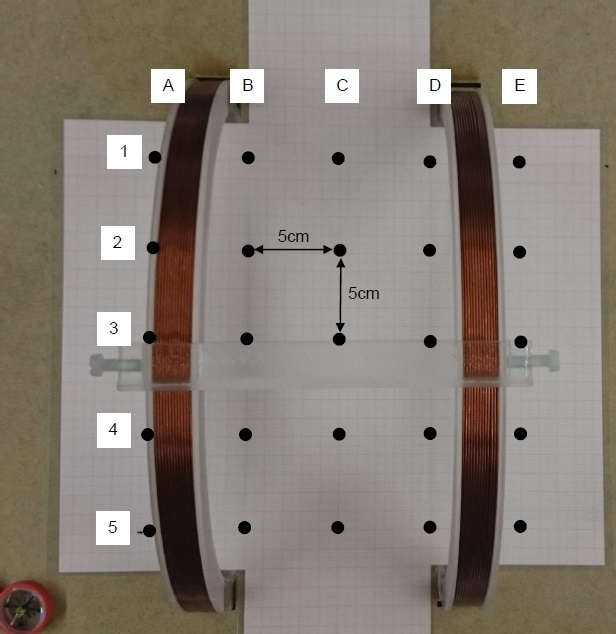
\includegraphics[scale=0.8]{Mess.pdf} 
	\caption{Grafische Übersicht der Messpunkte}
\end{figure}
\newpage
\subsubsection{Gleichgerichteter Stromfluss}
\paragraph{Axiale Komponenten in Gaus}
\textbf{Auswertung}
\begin{table}[H]
	\centering
	\begin{tabular}{|l|l|l|l|l|l|}
		\hline
		~ & A     & B    & C     & D    & E     \\ \hline
		1 & 15.5  & 22.1 & 13.4  & 21.7 & 13.9  \\ 
		2 & 14.4  & 17.4 & 16.5  & 16.9 & 13.4  \\ 
		3 & 16.6  & 16.5 & 16.6  & 16.0 & 13.1  \\ 
		4 & 14.1  & 16.4 & 16.4  & 16.8 & 13.75 \\ 
		5 & 14.3  & 13.2 & 13.21 & 21.0 & 14.81 \\
		\hline
	\end{tabular}
\begin{figure}[H]
	\centering
	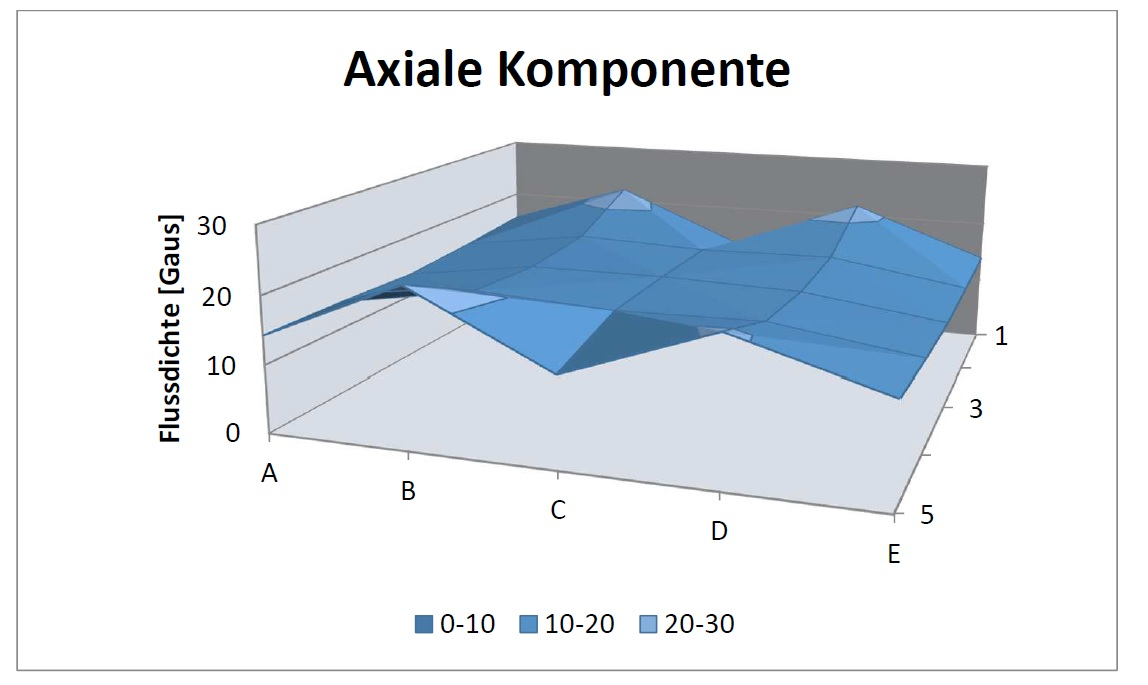
\includegraphics[scale=0.4]{GA.pdf} 
	\caption{Auswertung Axialer Komponenten}
\end{figure}
\end{table}
\newpage
\paragraph{Radiale Komponenten in Gaus}
\textbf{Auswertung}
\begin{table}[H]
	\centering
	\begin{tabular}{|l|l|l|l|l|l|}
		\hline
		~ & A    & B    & C    & D     & E    \\ \hline
		1 & -8.9 & 3.6  & 0.8  & -4,38 & 9.1  \\ 
		2 & -3.2 & 0    & 1.0  & 0.1   & 3.25 \\ 
		3 & -0.1 & 0    & 0.3  & -0.2  & 0.25 \\ 
		4 & 2    & 0    & 0.5  & -0.1  & -2.1 \\ 
		5 & 9.4  & -3,7 & -0.1 & 4.3   & -7,8 \\
		\hline
	\end{tabular}
\end{table}
\begin{figure}[H]
	\centering
	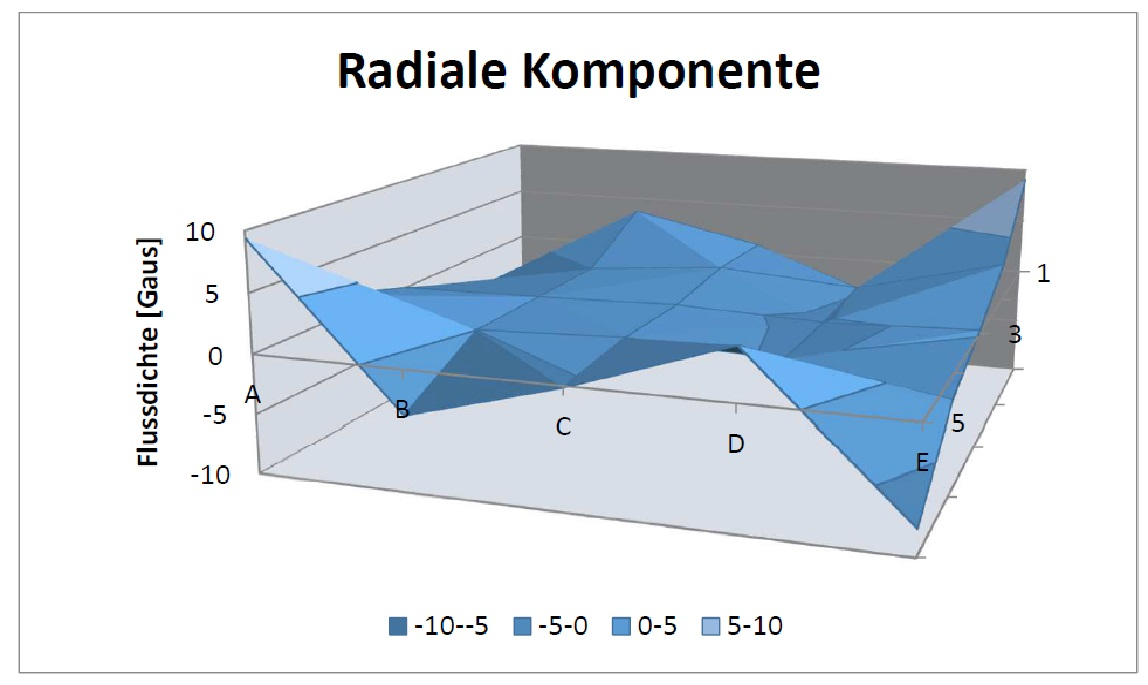
\includegraphics[scale=0.4]{GR.pdf} 
	\caption{Auswertung Radialer Komponenten}
\end{figure}
\newpage
\subsubsection{Gegengerichteter Stromfluss}
\paragraph{Axiale Komponenten in Gaus}
\textbf{Auswertung}
\begin{table}[H]
	\centering
	\begin{tabular}{|l|l|l|l|l|l|}
		\hline
		~ & A   & B    & C   & D     & E     \\ \hline
		1 & 11  & 1.5  & 0.3 & -13,8 & -9.4  \\ 
		2 & 8.7 & 8    & 0.5 & -6,9  & -7.5  \\ 
		3 & 7.7 & 6.6  & 0.1 & -5.4  & -6.7  \\ 
		4 & 8.7 & 8.5  & 0.2 & -8,8  & -7.8  \\ 
		5 & 9.9 & 16.4 & 0   & 13.4  & -10.4 \\
		\hline
	\end{tabular}
\end{table}
\begin{figure}[H]
	\centering
	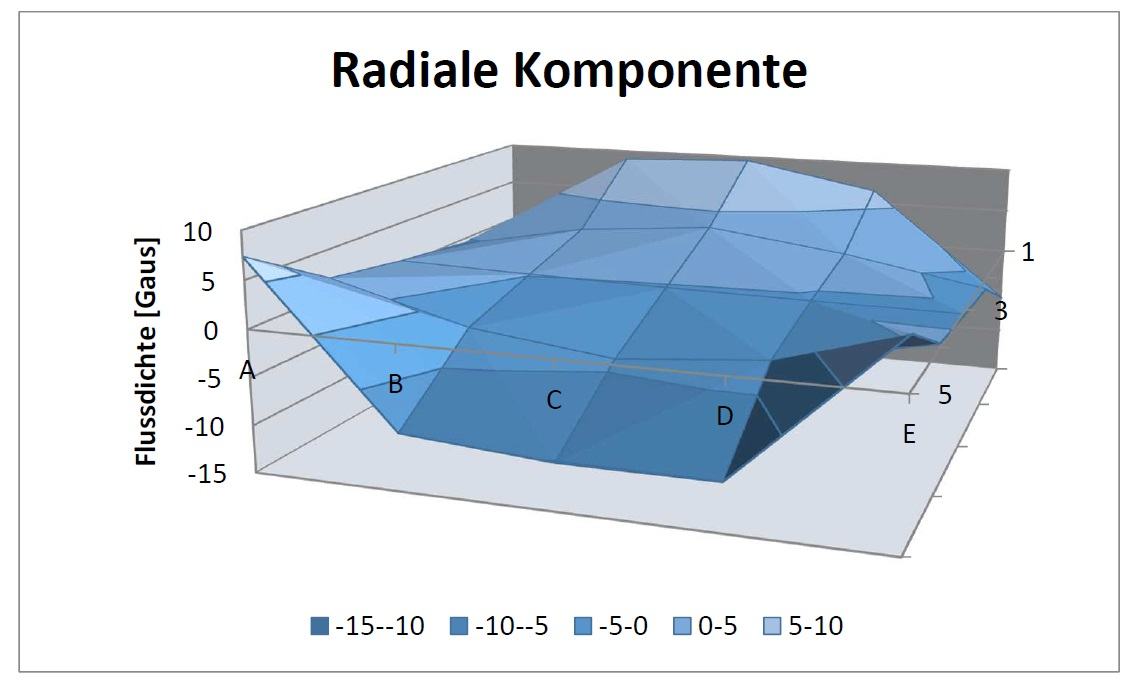
\includegraphics[scale=0.4]{BA.pdf} 
	\caption{Auswertung Axialer Komponenten}
\end{figure}
\newpage
\paragraph{Radiale Komponenten in Gaus}\textbf{Auswertung}
\begin{table}[H]
	\centering
	\begin{tabular}{|l|l|l|l|l|l|}
		\hline
		~ & A    & B    & C     & D    & E    \\ \hline
		1 & -4.7 & 8.9  & 9.5   & 6.5  & -5.9 \\ 
		2 & -0.5 & 2.4  & 3.7   & 1.6  & -1.3 \\ 
		3 & 0.5  & 0.2  & -0.2  & -0.4 & -0.5 \\ 
		4 & 1.8  & -2.2 & -4.2  & -2.8 & 0.4  \\ 
		5 & 7,3  & -9   & .10.1 & -10  & 5.3  \\
		\hline
	\end{tabular}
\end{table}
\begin{figure}[H]
	\centering
	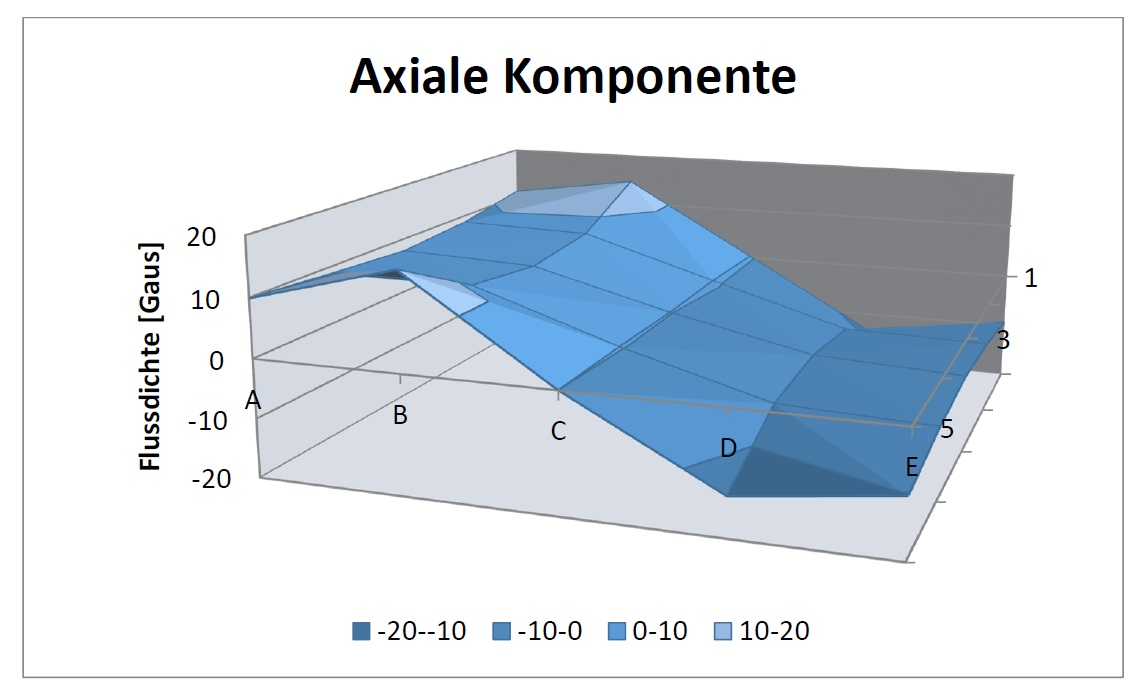
\includegraphics[scale=0.4]{BR.pdf} 
	\caption{Auswertung Radialer Komponenten}
\end{figure}
\section{Schlussfolgerung}
Auf den Bildern ist sehr schön zu erkennen, in welche Richtung das Magnetfeld geht. Es ist eine grosse Hilfe für das Verständnis.
\end{document}